\section{Выбор структуры и оптимальных параметров пневмопривода}\label{sec:inverse_optimization}

Построенные фронты Парето устанавливают предельно достижимые значения
критериев качества для каждой структуры. Для примера на рисунке \ref{fig:pareto_fronts_two}
изображены фронты Парето, соответствующие двум структурам пневмопривода (УСР-И-7 и УСР-Т-7)
и построенные для двух показателей качества $SI$ и $ITAE$ при $AC = \num{0.6}\text{мм}$. Оптимальное решение
всегда лежит на поверхности, огибающей фронты Парето. Выбор
структуры связан с поиском проектировщиком наиболее приемлемого сочетания
показателей качества на этой огибающей и определения структуры, чей фронт
Парето включает точку, соответствующую этому сочетанию.

\begin{figure}[h]
	\centering
	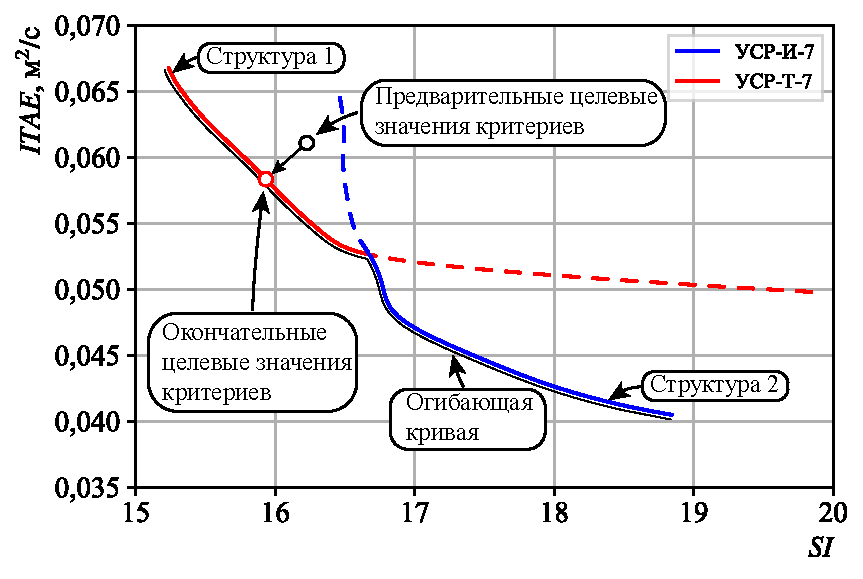
\includegraphics{part5/contour_comparison.pdf}
	\caption{Фронты Парето для двух структур пневмопривода}
	\label{fig:pareto_fronts_two}
\end{figure}
	

Данный подход позволяет проектировщику наглядно видеть цену
увеличения того или иного показателя качества за счет снижения
остальных, что позволяет более обоснованно назначать их целевые
значения. Кроме того, возможно улучшение предварительно заданных
целевых значений критериев качества до их предельно достижимых уровней.

Выбор окончательных целевых значений критериев качества может
быть осуществлено нахождением ближайшей точки на огибающей фронтов
Парето от точки, соответствующей предварительно назначенным целевым значениям (рисунок \ref{fig:pareto_fronts_two}).

Поскольку критерии имеют различную физическую природу и масштабы, для корректного определения
расстояния необходимо выполнить их нормализацию.
В данной работе используется нормализация относительно диапазона изменения каждого критерия:

\begin{equation}\label{eq:normalization}
	\tilde{y}_i = \frac{y_i - y_{i,\min}}{y_{i,\max} - y_{i,\min}}, \quad i \in \{AC, ITAE, SI\},
\end{equation}
где $y_{i,\min}$ и $y_{i,\max}$ -- минимальное и максимальное значения $i$-го критерия на фронте Парето.

В качестве меры расстояния между нормализованными векторами критериев используется взвешенная евклидова норма:

\begin{equation}\label{eq:weighted_norm}
	\|\mathbf{\tilde{y}}(\mathbf{p}) - \mathbf{\tilde{y}}^*\|_w = \sqrt{\sum_{i} w_i (\tilde{y}_i(\mathbf{p}) - \tilde{y}_i^*)^2},
\end{equation}
где $w_i$ -- весовые коэффициенты, отражающие относительную важность критериев.

Для практической реализации описанной выше методики разработан алгоритм поиска ближайшей точки
на фронте Парето к заданной целевой точке. Алгоритм включает предварительную обработку данных,
эффективный поиск ближайшей точки и дополнительную интерполяцию для повышения точности.

Перед началом поиска выполняется предварительная обработка данных, включающая следующие шаги:
\begin{enumerate}
	\item Фильтрация точек фронта Парето для исключения доминируемых точек, которые
	      могли появиться из-за численных погрешностей в процессе построения фронта.

	\item Вычисление диапазонов изменения критериев $[y_{i,\min}, y_{i,\max}]$ для каждого критерия $i$.
	\item Нормализация критериев для всех точек фронта Парето и целевой точки согласно уравнению~\eqref{eq:normalization}.
	\item Формирование пространственной структуры данных для эффективного поиска ближайших точек.
\end{enumerate}

Поиск ближайшей к целевой точки на фронте Парето осуществляется в два этапа:

\begin{enumerate}
	\item Грубый поиск -- вычисление расстояний от целевой точки до всех точек фронта Парето
	      и выбор точки с минимальным расстоянием. Этот этап необходим для определения начального приближения.
	\item Уточняющий поиск -- локальная оптимизация в окрестности найденной точки с использованием
	      кубической интерполяции. Данный этап позволяет более точно определить параметры управления в
	      случае, если оптимальное решение находится между точками фронта Парето.
\end{enumerate}

Для грубого поиска используется прямое вычисление расстояний по формуле~\eqref{eq:weighted_norm} и выбор точки с минимальным значением:

\begin{equation}\label{eq:brute_force_search}
	j^* = \arg\min_{j \in \{1,\ldots,N\}} \|\mathbf{\tilde{y}}^{(j)} - \mathbf{\tilde{y}}^*\|_w,
\end{equation}
где $\mathbf{\tilde{y}}^{(j)}$ -- вектор нормализованных критериев для $j$-й точки фронта Парето;
$N$ -- общее число точек на фронте.

Для уточняющего поиска используется квадратичная интерполяция параметров управления в
окрестности найденной точки. Пусть $\mathbf{p}^{(j^*)}$ -- вектор параметров управления;
соответствующий найденной ближайшей точке фронта Парето.
Тогда интерполированные параметры вычисляются следующим образом:

\begin{equation}\label{eq:interpolation}
	\mathbf{p}^* = \mathbf{p}^{(j^*)} + \sum_{k \in K} \alpha_k (\mathbf{p}^{(k)} - \mathbf{p}^{(j^*)}),
\end{equation}
где $K$ -- множество индексов ближайших соседей точки $j^*$;
$\alpha_k$ -- весовые коэффициенты, определяемые на основе расстояний до целевой точки:

\begin{equation}\label{eq:interpolation_weights}
	\alpha_k = \frac{(d_{j^*} - d_{\min})^2}{\sum_{l \in K} (d_l - d_{\min})^2} \cdot \frac{d_{\min}}{d_k},
\end{equation}
где $d_k = \|\mathbf{\tilde{y}}^{(k)} - \mathbf{\tilde{y}}^*\|_w$ -- расстояние от $k$-й точки до целевой точки;
$d_{\min} = \min_{k \in K} d_k$ -- минимальное расстояние среди рассматриваемых точек.

Найденное положение точки с окончательными целевыми значениями
критериев качества на огибающей кривой может быть уточнено экспертно.
Данное положение однозначно определяет наиболее предпочтительную структуру
по принадлежности этой точки фронту Парето той или иной структуры. 

Далее для выбранной структуры и вектора целевых значений критериев качества
требуется найти соответствующий вектор параметров оптимизации. 
Поскольку при построении фронта Парето было получено соответствие
рассчитанных точек фронта Парето и параметров оптимизации, то решение
этой задачи сводится к построению интерполяционной зависимости и
нахождению по ней значений параметров по известным значениям критериев качества.

После определения оптимальных значений параметров целесообразно провести перерасчет
критериев качества по исходной модели. Если полученные в результате моделирования значения
критериев существенно отличаются от целевых, что может быть вызвано нелинейностью зависимостей
между параметрами и критериями, выполняется коррекция параметров.

Коррекция основана на методе последовательных приближений:

\begin{equation}\label{eq:parameters_correction}
	\mathbf{p}^{(n+1)} = \mathbf{p}^{(n)} + \beta (\mathbf{y}^* - \mathbf{y}^{(n)}) \cdot \frac{\partial \mathbf{y}}{\partial \mathbf{p}}|_{\mathbf{p}^{(n)}},
\end{equation}
где $\mathbf{p}^{(n)}$ -- вектор параметров на $n$-й итерации;
$\mathbf{y}^{(n)}$ -- соответствующий вектор критериев;
$\beta$ -- коэффициент коррекции.
$\frac{\partial \mathbf{y}}{\partial \mathbf{p}}|_{\mathbf{p}^{(n)}}$ -- матрица частных производных критериев по параметрам, оцениваемая численно.
\nomenclature{$\mathbf{y}^{(n)}$}{Вектор критериев на $n$-й итерации\nomrefeqpage}
\nomenclature{$\frac{\partial \mathbf{y}}{\partial \mathbf{p}}|_{\mathbf{p}^{(n)}}$}{Матрица частных производных критериев по параметрам\nomrefeqpage}
\nomenclature{$\beta$}{Коррекционный коэффициент\nomrefeqpage}
\nomenclature{$\mathbf{p}^{(n+1)}$}{Вектор параметров на $(n+1)$-й итерации\nomrefeqpage}

Итерационный процесс коррекции продолжается до тех пор, пока не будет достигнута
требуемая точность соответствия критериев целевым значениям или не будет выполнено максимальное число итераций.